\section{Introducción}
\label{sec:introduccion}

En el ámbito de la ingeniería y la física aplicada, las \textit{coilguns}, también conocidas como \textit{lanzaderas electromagnéticas}, representan una tecnología de creciente interés debido a su potencial en aplicaciones tanto industriales como militares. El concepto de las lanzaderas electromagnéticas se origina en el siglo XIX, cuando se empiezan a explorar las propiedades del electromagnetismo y sus potenciales aplicaciones. Uno de los nombres con los que uno se puede referir a esta tecnología es \textit{Cañones de Gauss}, debido a que fue el matemático Carl Friedrich Gauss quién desarrolló en esta época las ecuaciones que regían el comportamiento del dispositivo. Sin embargo, no es hasta los tempranos años del siglo XX cuando se construye la primera lanzadera funcional, producto del ingenio del científico noruego Kristian Birkeland\citep{introCoilGun}.

\begin{figure}[h]
    \centering
    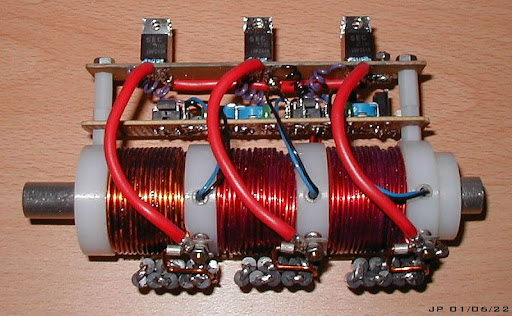
\includegraphics[width=7cm]{FigurasMemoria/fig1coilgunIntro.jpeg}
    \caption{Cañón de Gauss\citep{coilgun2024}.}
    \label{fig:prototipolanzadera} %Para referenciar -> \ref{fig:figNum}
\end{figure}

Las principales aplicaciones de las lanzaderas electromagnéticas se encuentran en el ámbito militar\citep{inproceedings}, donde se utilizan para el lanzamiento de proyectiles a alta velocidad sin la necesidad de explosivos químicos. Esta tecnología ofrece ventajas significativas, como la reducción del desgaste mecánico y la capacidad de ajustar la fuerza de lanzamiento con precisión. Además, en el sector aeroespacial\citep{inproceedings}, las lanzaderas electromagnéticas se consideran una alternativa prometedora para el lanzamiento de satélites y otros objetos al espacio, debido a su eficiencia energética y menor impacto ambiental en comparación con los cohetes tradicionales. También encontramos varias aplicaciones en la industria, como por ejemplo en procesos de manufactura que requieren la propulsión de materiales a altas velocidades. También se están explorando aplicaciones en el campo de la medicina, como en dispositivos de resonancia magnética y aceleradores de partículas para tratamientos médicos avanzados\citep{inproceedings}.

Para finalizar con la introducción, se presentará brevemente el funcionamiento básico de estos cañones. El objetivo físico de una lanzadera electromagnética es la creación de un campo magnético mediante el paso de una corriente eléctrica a través de una bobina de cobre. Cuando se aplica corriente a la bobina, se genera un campo magnético que ejerce una fuerza de atracción sobre el proyectil, que debe ser de material ferromagnético, al que me referiré durante este proyecto como \textbf{vástago}. El proceso de aceleración comienza cuando la corriente eléctrica, controlada por un circuito electrónico, fluye a través de la bobina, creando un campo magnético que atrae el proyectil hacia el centro de la bobina. Antes de que los centros de la bobina y el vástago estén alineados, la corriente se corta, provocando que este último continúe su movimiento hacia adelante debido a su inercia.

\newpage